
\section{Problem description}

One method of studying the input/output relationship of computer simulations 
is known as the 
\emph{black-box model}. 
The black-box in this case refers to the simulation code itself.
The simulation code is complex and expensive to run
so direct analysis is difficult.
Under this analysis method one does not make any assumptions as to the
inner workings of the simulation code.  Instead, we model the simulator as an
unknown continuous function
that takes a number
of numerical inputs and produces a number of numerical outputs.  We know
the domain of the inputs.  We want to study how varying the inputs
affects the output. 

While we don't know anything about how the simulation works internally, we can  
sample it by selecting a particular input setting through the simulation 
and recording the outputs.  We can then use a continuous reconstruction
method built from a number of samples in order to estimate the 
\emph{response surface}.
This fitted continuous function
is known as an \emph{emulator} in the
statistics literature.  We can then study the input/output relationship
using the emulator instead.  

\subsection{1D analysis example}
\label{sec:1d_example}

A common choice in the statistics community for this emulator is known as the
Gaussian process model~\cite{Rasmussen:2006}.  
One advantage of the Gaussian process model is that the form is very well
known and easy to analyze.  
It also allows us to measure the uncertainty of the estimation.
In order to illustrate the 
advantages we will go through a 1D example here using a known function
$f(x) = \sin(x) + \cos(2x)$
as a stand-in for some simulation code.

We begin by taking a number of discrete samples of the function.  Ideally
we take as many as possible but this may be limited in terms of time or
budget.  Since we do not know anything about the behavior of the function 
in the region we are sampling,
we sample in some uniform random fashion.
The function as well as the sample locations are shown in 
\autoref{fig:reconstruction_sampling}.

\begin{figure}[htb]
  \centering
  % Created by tikzDevice version 0.7.0 on 2014-07-31 11:04:19
% !TEX encoding = UTF-8 Unicode
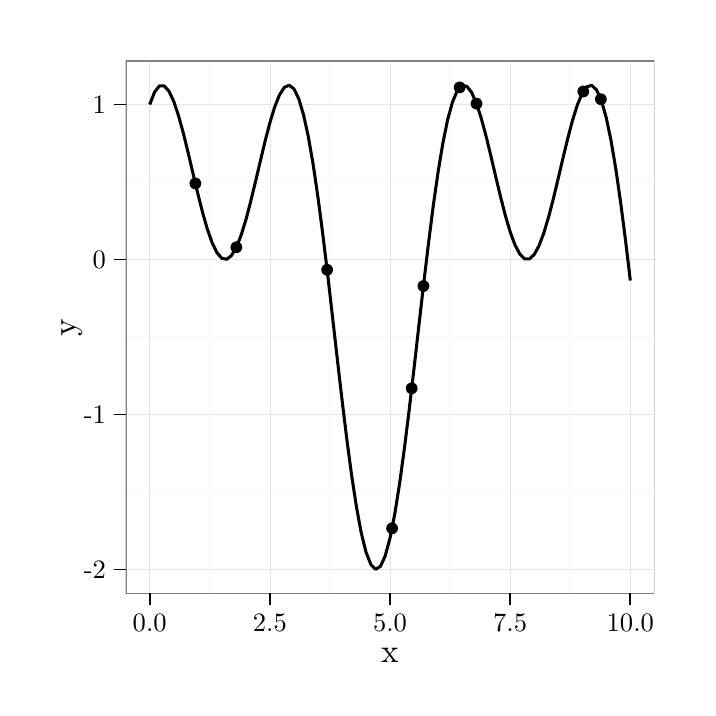
\begin{tikzpicture}[x=1pt,y=1pt]
\definecolor[named]{fillColor}{rgb}{1.00,1.00,1.00}
\path[use as bounding box,fill=fillColor,fill opacity=0.00] (0,0) rectangle (238.49,238.49);
\begin{scope}
\path[clip] (  0.00,  0.00) rectangle (238.49,238.49);
\definecolor[named]{drawColor}{rgb}{1.00,1.00,1.00}
\definecolor[named]{fillColor}{rgb}{1.00,1.00,1.00}

\path[draw=drawColor,line width= 0.6pt,line join=round,line cap=round,fill=fillColor] (  0.00,  0.00) rectangle (238.49,238.49);
\end{scope}
\begin{scope}
\path[clip] ( 35.42, 34.03) rectangle (226.45,226.45);
\definecolor[named]{fillColor}{rgb}{1.00,1.00,1.00}

\path[fill=fillColor] ( 35.42, 34.03) rectangle (226.45,226.45);
\definecolor[named]{drawColor}{rgb}{0.98,0.98,0.98}

\path[draw=drawColor,line width= 0.6pt,line join=round] ( 35.42, 70.75) --
	(226.45, 70.75);

\path[draw=drawColor,line width= 0.6pt,line join=round] ( 35.42,126.74) --
	(226.45,126.74);

\path[draw=drawColor,line width= 0.6pt,line join=round] ( 35.42,182.72) --
	(226.45,182.72);

\path[draw=drawColor,line width= 0.6pt,line join=round] ( 65.81, 34.03) --
	( 65.81,226.45);

\path[draw=drawColor,line width= 0.6pt,line join=round] (109.23, 34.03) --
	(109.23,226.45);

\path[draw=drawColor,line width= 0.6pt,line join=round] (152.64, 34.03) --
	(152.64,226.45);

\path[draw=drawColor,line width= 0.6pt,line join=round] (196.06, 34.03) --
	(196.06,226.45);
\definecolor[named]{drawColor}{rgb}{0.90,0.90,0.90}

\path[draw=drawColor,line width= 0.2pt,line join=round] ( 35.42, 42.76) --
	(226.45, 42.76);

\path[draw=drawColor,line width= 0.2pt,line join=round] ( 35.42, 98.74) --
	(226.45, 98.74);

\path[draw=drawColor,line width= 0.2pt,line join=round] ( 35.42,154.73) --
	(226.45,154.73);

\path[draw=drawColor,line width= 0.2pt,line join=round] ( 35.42,210.71) --
	(226.45,210.71);

\path[draw=drawColor,line width= 0.2pt,line join=round] ( 44.10, 34.03) --
	( 44.10,226.45);

\path[draw=drawColor,line width= 0.2pt,line join=round] ( 87.52, 34.03) --
	( 87.52,226.45);

\path[draw=drawColor,line width= 0.2pt,line join=round] (130.93, 34.03) --
	(130.93,226.45);

\path[draw=drawColor,line width= 0.2pt,line join=round] (174.35, 34.03) --
	(174.35,226.45);

\path[draw=drawColor,line width= 0.2pt,line join=round] (217.76, 34.03) --
	(217.76,226.45);
\definecolor[named]{drawColor}{rgb}{0.00,0.00,0.00}

\path[draw=drawColor,line width= 1.1pt,line join=round] ( 44.10,210.71) --
	( 45.84,215.19) --
	( 47.58,217.42) --
	( 49.31,217.48) --
	( 51.05,215.54) --
	( 52.79,211.82) --
	( 54.52,206.63) --
	( 56.26,200.31) --
	( 58.00,193.26) --
	( 59.73,185.86) --
	( 61.47,178.54) --
	( 63.21,171.68) --
	( 64.94,165.63) --
	( 66.68,160.70) --
	( 68.42,157.15) --
	( 70.15,155.15) --
	( 71.89,154.80) --
	( 73.63,156.12) --
	( 75.36,159.05) --
	( 77.10,163.43) --
	( 78.84,169.04) --
	( 80.57,175.61) --
	( 82.31,182.79) --
	( 84.05,190.20) --
	( 85.78,197.44) --
	( 87.52,204.12) --
	( 89.26,209.82) --
	( 90.99,214.19) --
	( 92.73,216.90) --
	( 94.47,217.70) --
	( 96.20,216.39) --
	( 97.94,212.85) --
	( 99.67,207.07) --
	(101.41,199.10) --
	(103.15,189.10) --
	(104.88,177.30) --
	(106.62,164.01) --
	(108.36,149.62) --
	(110.09,134.54) --
	(111.83,119.25) --
	(113.57,104.21) --
	(115.30, 89.93) --
	(117.04, 76.86) --
	(118.78, 65.44) --
	(120.51, 56.04) --
	(122.25, 48.99) --
	(123.99, 44.52) --
	(125.72, 42.78) --
	(127.46, 43.83) --
	(129.20, 47.64) --
	(130.93, 54.07) --
	(132.67, 62.91) --
	(134.41, 73.86) --
	(136.14, 86.56) --
	(137.88,100.59) --
	(139.62,115.48) --
	(141.35,130.75) --
	(143.09,145.93) --
	(144.83,160.53) --
	(146.56,174.13) --
	(148.30,186.33) --
	(150.04,196.80) --
	(151.77,205.29) --
	(153.51,211.62) --
	(155.25,215.72) --
	(156.98,217.58) --
	(158.72,217.29) --
	(160.46,215.03) --
	(162.19,211.04) --
	(163.93,205.63) --
	(165.67,199.17) --
	(167.40,192.03) --
	(169.14,184.62) --
	(170.88,177.34) --
	(172.61,170.59) --
	(174.35,164.71) --
	(176.08,160.00) --
	(177.82,156.70) --
	(179.56,154.97) --
	(181.29,154.91) --
	(183.03,156.50) --
	(184.77,159.69) --
	(186.50,164.29) --
	(188.24,170.09) --
	(189.98,176.78) --
	(191.71,184.03) --
	(193.45,191.44) --
	(195.19,198.62) --
	(196.92,205.15) --
	(198.66,210.66) --
	(200.40,214.77) --
	(202.13,217.18) --
	(203.87,217.63) --
	(205.61,215.95) --
	(207.34,212.03) --
	(209.08,205.88) --
	(210.82,197.55) --
	(212.55,187.23) --
	(214.29,175.16) --
	(216.03,161.66) --
	(217.76,147.12);
\definecolor[named]{fillColor}{rgb}{0.00,0.00,0.00}

\path[fill=fillColor] (207.13,212.64) circle (  2.13);

\path[fill=fillColor] (138.77,108.17) circle (  2.13);

\path[fill=fillColor] (162.19,211.04) circle (  2.13);

\path[fill=fillColor] (200.77,215.44) circle (  2.13);

\path[fill=fillColor] (143.00,145.13) circle (  2.13);

\path[fill=fillColor] (156.10,216.91) circle (  2.13);

\path[fill=fillColor] (131.68, 57.58) circle (  2.13);

\path[fill=fillColor] ( 75.41,159.14) circle (  2.13);

\path[fill=fillColor] ( 60.60,182.20) circle (  2.13);

\path[fill=fillColor] (108.20,151.00) circle (  2.13);
\definecolor[named]{drawColor}{rgb}{0.50,0.50,0.50}

\path[draw=drawColor,line width= 0.6pt,line join=round,line cap=round] ( 35.42, 34.03) rectangle (226.45,226.45);
\end{scope}
\begin{scope}
\path[clip] (  0.00,  0.00) rectangle (238.49,238.49);
\definecolor[named]{drawColor}{rgb}{0.00,0.00,0.00}

\node[text=drawColor,anchor=base east,inner sep=0pt, outer sep=0pt, scale=  0.96] at ( 28.31, 39.45) {-2};

\node[text=drawColor,anchor=base east,inner sep=0pt, outer sep=0pt, scale=  0.96] at ( 28.31, 95.44) {-1};

\node[text=drawColor,anchor=base east,inner sep=0pt, outer sep=0pt, scale=  0.96] at ( 28.31,151.42) {0};

\node[text=drawColor,anchor=base east,inner sep=0pt, outer sep=0pt, scale=  0.96] at ( 28.31,207.41) {1};
\end{scope}
\begin{scope}
\path[clip] (  0.00,  0.00) rectangle (238.49,238.49);
\definecolor[named]{drawColor}{rgb}{0.00,0.00,0.00}

\path[draw=drawColor,line width= 0.6pt,line join=round] ( 31.15, 42.76) --
	( 35.42, 42.76);

\path[draw=drawColor,line width= 0.6pt,line join=round] ( 31.15, 98.74) --
	( 35.42, 98.74);

\path[draw=drawColor,line width= 0.6pt,line join=round] ( 31.15,154.73) --
	( 35.42,154.73);

\path[draw=drawColor,line width= 0.6pt,line join=round] ( 31.15,210.71) --
	( 35.42,210.71);
\end{scope}
\begin{scope}
\path[clip] (  0.00,  0.00) rectangle (238.49,238.49);
\definecolor[named]{drawColor}{rgb}{0.00,0.00,0.00}

\path[draw=drawColor,line width= 0.6pt,line join=round] ( 44.10, 29.77) --
	( 44.10, 34.03);

\path[draw=drawColor,line width= 0.6pt,line join=round] ( 87.52, 29.77) --
	( 87.52, 34.03);

\path[draw=drawColor,line width= 0.6pt,line join=round] (130.93, 29.77) --
	(130.93, 34.03);

\path[draw=drawColor,line width= 0.6pt,line join=round] (174.35, 29.77) --
	(174.35, 34.03);

\path[draw=drawColor,line width= 0.6pt,line join=round] (217.76, 29.77) --
	(217.76, 34.03);
\end{scope}
\begin{scope}
\path[clip] (  0.00,  0.00) rectangle (238.49,238.49);
\definecolor[named]{drawColor}{rgb}{0.00,0.00,0.00}

\node[text=drawColor,anchor=base,inner sep=0pt, outer sep=0pt, scale=  0.96] at ( 44.10, 20.31) {0.0};

\node[text=drawColor,anchor=base,inner sep=0pt, outer sep=0pt, scale=  0.96] at ( 87.52, 20.31) {2.5};

\node[text=drawColor,anchor=base,inner sep=0pt, outer sep=0pt, scale=  0.96] at (130.93, 20.31) {5.0};

\node[text=drawColor,anchor=base,inner sep=0pt, outer sep=0pt, scale=  0.96] at (174.35, 20.31) {7.5};

\node[text=drawColor,anchor=base,inner sep=0pt, outer sep=0pt, scale=  0.96] at (217.76, 20.31) {10.0};
\end{scope}
\begin{scope}
\path[clip] (  0.00,  0.00) rectangle (238.49,238.49);
\definecolor[named]{drawColor}{rgb}{0.00,0.00,0.00}

\node[text=drawColor,anchor=base,inner sep=0pt, outer sep=0pt, scale=  1.20] at (130.93,  9.03) {x};
\end{scope}
\begin{scope}
\path[clip] (  0.00,  0.00) rectangle (238.49,238.49);
\definecolor[named]{drawColor}{rgb}{0.00,0.00,0.00}

\node[text=drawColor,rotate= 90.00,anchor=base,inner sep=0pt, outer sep=0pt, scale=  1.20] at ( 17.30,130.24) {y};
\end{scope}
\end{tikzpicture}

  %\includegraphics[width=8cm]{example_function_sampled}
  \caption{
    An example of taking 10 uniformly distributed samples of the function
    $f(x) = sin(x) + cos(2x)$.  The dots show the sampling locations.
  }
  \label{fig:reconstruction_sampling}
\end{figure}

%Signal processing theory~\cite{Oppenheim:1999} gives the relationship between 
%the
%number of samples and how much frequency content we can glean from the signal.
We would prefer to take as many samples as possible in order to identify
the various peaks and valleys.
The interpolation method we choose depends on how we expect the values to
change between the sample points.
%\ttwnote{in signal processing  it depends on the number of samples taken and the continuity of the reconstruction but I don't quite understand\ldots}.  
If we expect linear behavior then fitting a
piecewise linear function would be ideal.  If we expect more complex behavior
then we should fit higher-order functions.  We show 3 different fitting 
methods for our function in \autoref{fig:interp_methods}: piecewise linear (blue), 
cubic spline (green), and Gaussian process model (red) along with the true
function (black).  In this case the cubic spline and Gaussian process model
interpolations are very close to the true function, but the true function
normally would not be known beforehand.

\begin{figure}[htb]
  \centering
  % Created by tikzDevice version 0.7.0 on 2014-07-31 11:04:27
% !TEX encoding = UTF-8 Unicode
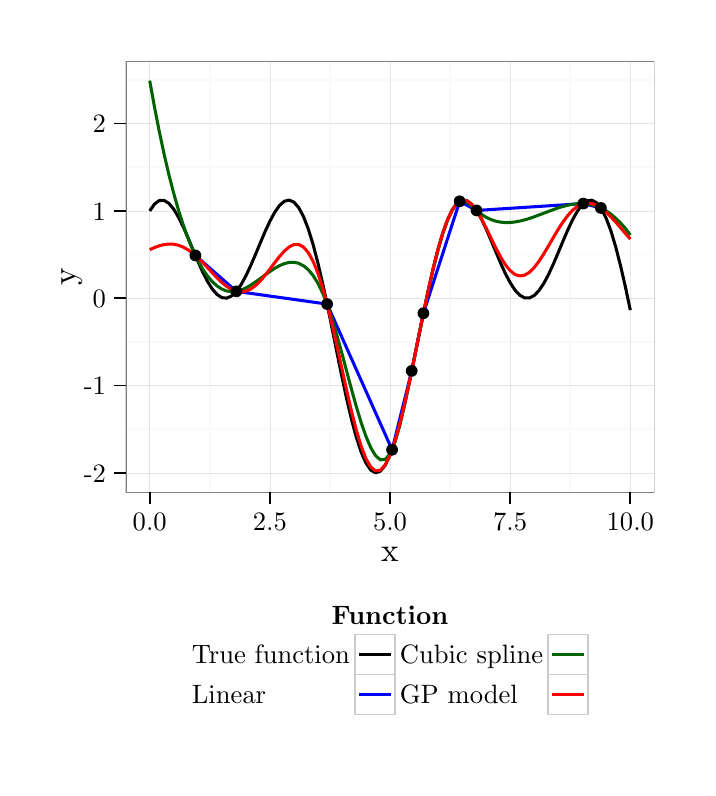
\begin{tikzpicture}[x=1pt,y=1pt]
\definecolor[named]{fillColor}{rgb}{1.00,1.00,1.00}
\path[use as bounding box,fill=fillColor,fill opacity=0.00] (0,0) rectangle (238.49,267.40);
\begin{scope}
\path[clip] (  0.00,  0.00) rectangle (238.49,267.40);
\definecolor[named]{drawColor}{rgb}{1.00,1.00,1.00}
\definecolor[named]{fillColor}{rgb}{1.00,1.00,1.00}

\path[draw=drawColor,line width= 0.6pt,line join=round,line cap=round,fill=fillColor] (  0.00,  0.00) rectangle (238.49,267.40);
\end{scope}
\begin{scope}
\path[clip] ( 35.42, 99.45) rectangle (226.45,255.35);
\definecolor[named]{fillColor}{rgb}{1.00,1.00,1.00}

\path[fill=fillColor] ( 35.42, 99.45) rectangle (226.45,255.35);
\definecolor[named]{drawColor}{rgb}{0.98,0.98,0.98}

\path[draw=drawColor,line width= 0.6pt,line join=round] ( 35.42,122.30) --
	(226.45,122.30);

\path[draw=drawColor,line width= 0.6pt,line join=round] ( 35.42,153.85) --
	(226.45,153.85);

\path[draw=drawColor,line width= 0.6pt,line join=round] ( 35.42,185.39) --
	(226.45,185.39);

\path[draw=drawColor,line width= 0.6pt,line join=round] ( 35.42,216.94) --
	(226.45,216.94);

\path[draw=drawColor,line width= 0.6pt,line join=round] ( 35.42,248.49) --
	(226.45,248.49);

\path[draw=drawColor,line width= 0.6pt,line join=round] ( 65.81, 99.45) --
	( 65.81,255.35);

\path[draw=drawColor,line width= 0.6pt,line join=round] (109.23, 99.45) --
	(109.23,255.35);

\path[draw=drawColor,line width= 0.6pt,line join=round] (152.64, 99.45) --
	(152.64,255.35);

\path[draw=drawColor,line width= 0.6pt,line join=round] (196.06, 99.45) --
	(196.06,255.35);
\definecolor[named]{drawColor}{rgb}{0.90,0.90,0.90}

\path[draw=drawColor,line width= 0.2pt,line join=round] ( 35.42,106.53) --
	(226.45,106.53);

\path[draw=drawColor,line width= 0.2pt,line join=round] ( 35.42,138.07) --
	(226.45,138.07);

\path[draw=drawColor,line width= 0.2pt,line join=round] ( 35.42,169.62) --
	(226.45,169.62);

\path[draw=drawColor,line width= 0.2pt,line join=round] ( 35.42,201.17) --
	(226.45,201.17);

\path[draw=drawColor,line width= 0.2pt,line join=round] ( 35.42,232.71) --
	(226.45,232.71);

\path[draw=drawColor,line width= 0.2pt,line join=round] ( 44.10, 99.45) --
	( 44.10,255.35);

\path[draw=drawColor,line width= 0.2pt,line join=round] ( 87.52, 99.45) --
	( 87.52,255.35);

\path[draw=drawColor,line width= 0.2pt,line join=round] (130.93, 99.45) --
	(130.93,255.35);

\path[draw=drawColor,line width= 0.2pt,line join=round] (174.35, 99.45) --
	(174.35,255.35);

\path[draw=drawColor,line width= 0.2pt,line join=round] (217.76, 99.45) --
	(217.76,255.35);
\definecolor[named]{drawColor}{rgb}{0.00,0.00,0.00}

\path[draw=drawColor,line width= 1.1pt,line join=round] ( 44.10,201.17) --
	( 45.84,203.69) --
	( 47.58,204.94) --
	( 49.31,204.98) --
	( 51.05,203.88) --
	( 52.79,201.79) --
	( 54.52,198.86) --
	( 56.26,195.31) --
	( 58.00,191.33) --
	( 59.73,187.16) --
	( 61.47,183.04) --
	( 63.21,179.17) --
	( 64.94,175.76) --
	( 66.68,172.99) --
	( 68.42,170.98) --
	( 70.15,169.86) --
	( 71.89,169.66) --
	( 73.63,170.41) --
	( 75.36,172.05) --
	( 77.10,174.52) --
	( 78.84,177.69) --
	( 80.57,181.39) --
	( 82.31,185.43) --
	( 84.05,189.61) --
	( 85.78,193.69) --
	( 87.52,197.45) --
	( 89.26,200.66) --
	( 90.99,203.13) --
	( 92.73,204.66) --
	( 94.47,205.10) --
	( 96.20,204.36) --
	( 97.94,202.37) --
	( 99.67,199.11) --
	(101.41,194.62) --
	(103.15,188.99) --
	(104.88,182.34) --
	(106.62,174.85) --
	(108.36,166.74) --
	(110.09,158.25) --
	(111.83,149.63) --
	(113.57,141.16) --
	(115.30,133.11) --
	(117.04,125.74) --
	(118.78,119.31) --
	(120.51,114.01) --
	(122.25,110.04) --
	(123.99,107.52) --
	(125.72,106.54) --
	(127.46,107.13) --
	(129.20,109.28) --
	(130.93,112.90) --
	(132.67,117.88) --
	(134.41,124.05) --
	(136.14,131.21) --
	(137.88,139.11) --
	(139.62,147.50) --
	(141.35,156.11) --
	(143.09,164.66) --
	(144.83,172.89) --
	(146.56,180.55) --
	(148.30,187.43) --
	(150.04,193.33) --
	(151.77,198.11) --
	(153.51,201.68) --
	(155.25,203.99) --
	(156.98,205.03) --
	(158.72,204.87) --
	(160.46,203.60) --
	(162.19,201.35) --
	(163.93,198.30) --
	(165.67,194.66) --
	(167.40,190.64) --
	(169.14,186.46) --
	(170.88,182.36) --
	(172.61,178.56) --
	(174.35,175.25) --
	(176.08,172.59) --
	(177.82,170.73) --
	(179.56,169.76) --
	(181.29,169.72) --
	(183.03,170.62) --
	(184.77,172.41) --
	(186.50,175.01) --
	(188.24,178.28) --
	(189.98,182.05) --
	(191.71,186.13) --
	(193.45,190.31) --
	(195.19,194.35) --
	(196.92,198.03) --
	(198.66,201.14) --
	(200.40,203.45) --
	(202.13,204.81) --
	(203.87,205.06) --
	(205.61,204.12) --
	(207.34,201.91) --
	(209.08,198.44) --
	(210.82,193.75) --
	(212.55,187.93) --
	(214.29,181.13) --
	(216.03,173.53) --
	(217.76,165.33);
\definecolor[named]{drawColor}{rgb}{0.00,0.00,1.00}

\path[draw=drawColor,line width= 1.1pt,line join=round] ( 60.60,185.10) --
	( 75.41,172.11) --
	(108.20,167.52) --
	(131.68,114.88) --
	(138.77,143.38) --
	(143.00,164.21) --
	(156.10,204.66) --
	(162.19,201.35) --
	(200.77,203.83) --
	(207.13,202.25);
\definecolor[named]{drawColor}{rgb}{0.00,0.39,0.00}

\path[draw=drawColor,line width= 1.1pt,line join=round] ( 44.10,248.27) --
	( 45.84,238.63) --
	( 47.58,229.76) --
	( 49.31,221.63) --
	( 51.05,214.20) --
	( 52.79,207.47) --
	( 54.52,201.40) --
	( 56.26,195.98) --
	( 58.00,191.18) --
	( 59.73,186.97) --
	( 61.47,183.34) --
	( 63.21,180.25) --
	( 64.94,177.70) --
	( 66.68,175.64) --
	( 68.42,174.07) --
	( 70.15,172.95) --
	( 71.89,172.26) --
	( 73.63,171.99) --
	( 75.36,172.10) --
	( 77.10,172.57) --
	( 78.84,173.33) --
	( 80.57,174.33) --
	( 82.31,175.49) --
	( 84.05,176.74) --
	( 85.78,178.03) --
	( 87.52,179.28) --
	( 89.26,180.42) --
	( 90.99,181.40) --
	( 92.73,182.13) --
	( 94.47,182.57) --
	( 96.20,182.63) --
	( 97.94,182.25) --
	( 99.67,181.38) --
	(101.41,179.92) --
	(103.15,177.83) --
	(104.88,175.04) --
	(106.62,171.47) --
	(108.36,167.07) --
	(110.09,161.82) --
	(111.83,155.93) --
	(113.57,149.61) --
	(115.30,143.10) --
	(117.04,136.62) --
	(118.78,130.40) --
	(120.51,124.68) --
	(122.25,119.67) --
	(123.99,115.61) --
	(125.72,112.73) --
	(127.46,111.24) --
	(129.20,111.39) --
	(130.93,113.39) --
	(132.67,117.46) --
	(134.41,123.42) --
	(136.14,130.76) --
	(137.88,138.98) --
	(139.62,147.58) --
	(141.35,156.20) --
	(143.09,164.65) --
	(144.83,172.74) --
	(146.56,180.30) --
	(148.30,187.14) --
	(150.04,193.11) --
	(151.77,198.04) --
	(153.51,201.75) --
	(155.25,204.07) --
	(156.98,204.86) --
	(158.72,204.31) --
	(160.46,202.95) --
	(162.19,201.35) --
	(163.93,199.97) --
	(165.67,198.88) --
	(167.40,198.05) --
	(169.14,197.48) --
	(170.88,197.12) --
	(172.61,196.97) --
	(174.35,197.00) --
	(176.08,197.19) --
	(177.82,197.51) --
	(179.56,197.94) --
	(181.29,198.46) --
	(183.03,199.06) --
	(184.77,199.70) --
	(186.50,200.36) --
	(188.24,201.02) --
	(189.98,201.67) --
	(191.71,202.27) --
	(193.45,202.80) --
	(195.19,203.25) --
	(196.92,203.59) --
	(198.66,203.79) --
	(200.40,203.84) --
	(202.13,203.72) --
	(203.87,203.40) --
	(205.61,202.88) --
	(207.34,202.15) --
	(209.08,201.18) --
	(210.82,199.97) --
	(212.55,198.51) --
	(214.29,196.78) --
	(216.03,194.78) --
	(217.76,192.47);
\definecolor[named]{drawColor}{rgb}{1.00,0.00,0.00}

\path[draw=drawColor,line width= 1.1pt,line join=round] ( 44.10,187.19) --
	( 45.84,187.96) --
	( 47.58,188.58) --
	( 49.31,189.02) --
	( 51.05,189.21) --
	( 52.79,189.14) --
	( 54.52,188.77) --
	( 56.26,188.09) --
	( 58.00,187.10) --
	( 59.73,185.83) --
	( 61.47,184.30) --
	( 63.21,182.58) --
	( 64.94,180.74) --
	( 66.68,178.86) --
	( 68.42,177.03) --
	( 70.15,175.35) --
	( 71.89,173.92) --
	( 73.63,172.81) --
	( 75.36,172.12) --
	( 77.10,171.89) --
	( 78.84,172.16) --
	( 80.57,172.94) --
	( 82.31,174.19) --
	( 84.05,175.87) --
	( 85.78,177.89) --
	( 87.52,180.14) --
	( 89.26,182.46) --
	( 90.99,184.69) --
	( 92.73,186.66) --
	( 94.47,188.16) --
	( 96.20,189.02) --
	( 97.94,189.05) --
	( 99.67,188.12) --
	(101.41,186.11) --
	(103.15,182.96) --
	(104.88,178.65) --
	(106.62,173.26) --
	(108.36,166.89) --
	(110.09,159.73) --
	(111.83,152.03) --
	(113.57,144.07) --
	(115.30,136.18) --
	(117.04,128.67) --
	(118.78,121.89) --
	(120.51,116.13) --
	(122.25,111.64) --
	(123.99,108.64) --
	(125.72,107.24) --
	(127.46,107.51) --
	(129.20,109.43) --
	(130.93,112.93) --
	(132.67,117.86) --
	(134.41,124.02) --
	(136.14,131.19) --
	(137.88,139.11) --
	(139.62,147.51) --
	(141.35,156.12) --
	(143.09,164.66) --
	(144.83,172.88) --
	(146.56,180.54) --
	(148.30,187.42) --
	(150.04,193.33) --
	(151.77,198.13) --
	(153.51,201.70) --
	(155.25,204.00) --
	(156.98,205.02) --
	(158.72,204.84) --
	(160.46,203.56) --
	(162.19,201.35) --
	(163.93,198.43) --
	(165.67,195.03) --
	(167.40,191.42) --
	(169.14,187.85) --
	(170.88,184.56) --
	(172.61,181.76) --
	(174.35,179.61) --
	(176.08,178.23) --
	(177.82,177.68) --
	(179.56,177.95) --
	(181.29,179.00) --
	(183.03,180.73) --
	(184.77,183.01) --
	(186.50,185.70) --
	(188.24,188.62) --
	(189.98,191.62) --
	(191.71,194.53) --
	(193.45,197.21) --
	(195.19,199.55) --
	(196.92,201.45) --
	(198.66,202.85) --
	(200.40,203.72) --
	(202.13,204.04) --
	(203.87,203.85) --
	(205.61,203.18) --
	(207.34,202.10) --
	(209.08,200.66) --
	(210.82,198.95) --
	(212.55,197.06) --
	(214.29,195.05) --
	(216.03,193.00) --
	(217.76,190.98);
\definecolor[named]{fillColor}{rgb}{0.00,0.00,0.00}

\path[fill=fillColor] (207.13,202.25) circle (  2.13);

\path[fill=fillColor] (138.77,143.38) circle (  2.13);

\path[fill=fillColor] (162.19,201.35) circle (  2.13);

\path[fill=fillColor] (200.77,203.83) circle (  2.13);

\path[fill=fillColor] (143.00,164.21) circle (  2.13);

\path[fill=fillColor] (156.10,204.66) circle (  2.13);

\path[fill=fillColor] (131.68,114.88) circle (  2.13);

\path[fill=fillColor] ( 75.41,172.11) circle (  2.13);

\path[fill=fillColor] ( 60.60,185.10) circle (  2.13);

\path[fill=fillColor] (108.20,167.52) circle (  2.13);
\definecolor[named]{drawColor}{rgb}{0.50,0.50,0.50}

\path[draw=drawColor,line width= 0.6pt,line join=round,line cap=round] ( 35.42, 99.45) rectangle (226.45,255.35);
\end{scope}
\begin{scope}
\path[clip] (  0.00,  0.00) rectangle (238.49,267.40);
\definecolor[named]{drawColor}{rgb}{0.00,0.00,0.00}

\node[text=drawColor,anchor=base east,inner sep=0pt, outer sep=0pt, scale=  0.96] at ( 28.31,103.22) {-2};

\node[text=drawColor,anchor=base east,inner sep=0pt, outer sep=0pt, scale=  0.96] at ( 28.31,134.77) {-1};

\node[text=drawColor,anchor=base east,inner sep=0pt, outer sep=0pt, scale=  0.96] at ( 28.31,166.31) {0};

\node[text=drawColor,anchor=base east,inner sep=0pt, outer sep=0pt, scale=  0.96] at ( 28.31,197.86) {1};

\node[text=drawColor,anchor=base east,inner sep=0pt, outer sep=0pt, scale=  0.96] at ( 28.31,229.41) {2};
\end{scope}
\begin{scope}
\path[clip] (  0.00,  0.00) rectangle (238.49,267.40);
\definecolor[named]{drawColor}{rgb}{0.00,0.00,0.00}

\path[draw=drawColor,line width= 0.6pt,line join=round] ( 31.15,106.53) --
	( 35.42,106.53);

\path[draw=drawColor,line width= 0.6pt,line join=round] ( 31.15,138.07) --
	( 35.42,138.07);

\path[draw=drawColor,line width= 0.6pt,line join=round] ( 31.15,169.62) --
	( 35.42,169.62);

\path[draw=drawColor,line width= 0.6pt,line join=round] ( 31.15,201.17) --
	( 35.42,201.17);

\path[draw=drawColor,line width= 0.6pt,line join=round] ( 31.15,232.71) --
	( 35.42,232.71);
\end{scope}
\begin{scope}
\path[clip] (  0.00,  0.00) rectangle (238.49,267.40);
\definecolor[named]{drawColor}{rgb}{0.00,0.00,0.00}

\path[draw=drawColor,line width= 0.6pt,line join=round] ( 44.10, 95.18) --
	( 44.10, 99.45);

\path[draw=drawColor,line width= 0.6pt,line join=round] ( 87.52, 95.18) --
	( 87.52, 99.45);

\path[draw=drawColor,line width= 0.6pt,line join=round] (130.93, 95.18) --
	(130.93, 99.45);

\path[draw=drawColor,line width= 0.6pt,line join=round] (174.35, 95.18) --
	(174.35, 99.45);

\path[draw=drawColor,line width= 0.6pt,line join=round] (217.76, 95.18) --
	(217.76, 99.45);
\end{scope}
\begin{scope}
\path[clip] (  0.00,  0.00) rectangle (238.49,267.40);
\definecolor[named]{drawColor}{rgb}{0.00,0.00,0.00}

\node[text=drawColor,anchor=base,inner sep=0pt, outer sep=0pt, scale=  0.96] at ( 44.10, 85.73) {0.0};

\node[text=drawColor,anchor=base,inner sep=0pt, outer sep=0pt, scale=  0.96] at ( 87.52, 85.73) {2.5};

\node[text=drawColor,anchor=base,inner sep=0pt, outer sep=0pt, scale=  0.96] at (130.93, 85.73) {5.0};

\node[text=drawColor,anchor=base,inner sep=0pt, outer sep=0pt, scale=  0.96] at (174.35, 85.73) {7.5};

\node[text=drawColor,anchor=base,inner sep=0pt, outer sep=0pt, scale=  0.96] at (217.76, 85.73) {10.0};
\end{scope}
\begin{scope}
\path[clip] (  0.00,  0.00) rectangle (238.49,267.40);
\definecolor[named]{drawColor}{rgb}{0.00,0.00,0.00}

\node[text=drawColor,anchor=base,inner sep=0pt, outer sep=0pt, scale=  1.20] at (130.93, 74.45) {x};
\end{scope}
\begin{scope}
\path[clip] (  0.00,  0.00) rectangle (238.49,267.40);
\definecolor[named]{drawColor}{rgb}{0.00,0.00,0.00}

\node[text=drawColor,rotate= 90.00,anchor=base,inner sep=0pt, outer sep=0pt, scale=  1.20] at ( 17.30,177.40) {y};
\end{scope}
\begin{scope}
\path[clip] (  0.00,  0.00) rectangle (238.49,267.40);
\definecolor[named]{fillColor}{rgb}{1.00,1.00,1.00}

\path[fill=fillColor] ( 55.07, 14.89) rectangle (206.79, 62.57);
\end{scope}
\begin{scope}
\path[clip] (  0.00,  0.00) rectangle (238.49,267.40);
\definecolor[named]{drawColor}{rgb}{0.00,0.00,0.00}

\node[text=drawColor,anchor=base,inner sep=0pt, outer sep=0pt, scale=  0.96] at (130.93, 51.68) {\bfseries Function};
\end{scope}
\begin{scope}
\path[clip] (  0.00,  0.00) rectangle (238.49,267.40);
\definecolor[named]{drawColor}{rgb}{0.80,0.80,0.80}
\definecolor[named]{fillColor}{rgb}{1.00,1.00,1.00}

\path[draw=drawColor,line width= 0.6pt,line join=round,line cap=round,fill=fillColor] (118.23, 33.61) rectangle (132.68, 48.07);
\end{scope}
\begin{scope}
\path[clip] (  0.00,  0.00) rectangle (238.49,267.40);
\definecolor[named]{drawColor}{rgb}{0.00,0.00,0.00}

\path[draw=drawColor,line width= 1.1pt,line join=round] (119.67, 40.84) -- (131.24, 40.84);
\end{scope}
\begin{scope}
\path[clip] (  0.00,  0.00) rectangle (238.49,267.40);
\definecolor[named]{drawColor}{rgb}{0.00,0.00,0.00}

\path[draw=drawColor,line width= 1.1pt,line join=round] (119.67, 40.84) -- (131.24, 40.84);
\end{scope}
\begin{scope}
\path[clip] (  0.00,  0.00) rectangle (238.49,267.40);
\definecolor[named]{drawColor}{rgb}{0.00,0.00,0.00}

\path[draw=drawColor,line width= 1.1pt,line join=round] (119.67, 40.84) -- (131.24, 40.84);
\end{scope}
\begin{scope}
\path[clip] (  0.00,  0.00) rectangle (238.49,267.40);
\definecolor[named]{drawColor}{rgb}{0.00,0.00,0.00}

\path[draw=drawColor,line width= 1.1pt,line join=round] (119.67, 40.84) -- (131.24, 40.84);
\end{scope}
\begin{scope}
\path[clip] (  0.00,  0.00) rectangle (238.49,267.40);
\definecolor[named]{drawColor}{rgb}{0.80,0.80,0.80}
\definecolor[named]{fillColor}{rgb}{1.00,1.00,1.00}

\path[draw=drawColor,line width= 0.6pt,line join=round,line cap=round,fill=fillColor] (118.23, 19.16) rectangle (132.68, 33.61);
\end{scope}
\begin{scope}
\path[clip] (  0.00,  0.00) rectangle (238.49,267.40);
\definecolor[named]{drawColor}{rgb}{0.00,0.00,1.00}

\path[draw=drawColor,line width= 1.1pt,line join=round] (119.67, 26.39) -- (131.24, 26.39);
\end{scope}
\begin{scope}
\path[clip] (  0.00,  0.00) rectangle (238.49,267.40);
\definecolor[named]{drawColor}{rgb}{0.00,0.00,1.00}

\path[draw=drawColor,line width= 1.1pt,line join=round] (119.67, 26.39) -- (131.24, 26.39);
\end{scope}
\begin{scope}
\path[clip] (  0.00,  0.00) rectangle (238.49,267.40);
\definecolor[named]{drawColor}{rgb}{0.00,0.00,1.00}

\path[draw=drawColor,line width= 1.1pt,line join=round] (119.67, 26.39) -- (131.24, 26.39);
\end{scope}
\begin{scope}
\path[clip] (  0.00,  0.00) rectangle (238.49,267.40);
\definecolor[named]{drawColor}{rgb}{0.00,0.00,1.00}

\path[draw=drawColor,line width= 1.1pt,line join=round] (119.67, 26.39) -- (131.24, 26.39);
\end{scope}
\begin{scope}
\path[clip] (  0.00,  0.00) rectangle (238.49,267.40);
\definecolor[named]{drawColor}{rgb}{0.80,0.80,0.80}
\definecolor[named]{fillColor}{rgb}{1.00,1.00,1.00}

\path[draw=drawColor,line width= 0.6pt,line join=round,line cap=round,fill=fillColor] (188.07, 33.61) rectangle (202.52, 48.07);
\end{scope}
\begin{scope}
\path[clip] (  0.00,  0.00) rectangle (238.49,267.40);
\definecolor[named]{drawColor}{rgb}{0.00,0.39,0.00}

\path[draw=drawColor,line width= 1.1pt,line join=round] (189.52, 40.84) -- (201.08, 40.84);
\end{scope}
\begin{scope}
\path[clip] (  0.00,  0.00) rectangle (238.49,267.40);
\definecolor[named]{drawColor}{rgb}{0.00,0.39,0.00}

\path[draw=drawColor,line width= 1.1pt,line join=round] (189.52, 40.84) -- (201.08, 40.84);
\end{scope}
\begin{scope}
\path[clip] (  0.00,  0.00) rectangle (238.49,267.40);
\definecolor[named]{drawColor}{rgb}{0.00,0.39,0.00}

\path[draw=drawColor,line width= 1.1pt,line join=round] (189.52, 40.84) -- (201.08, 40.84);
\end{scope}
\begin{scope}
\path[clip] (  0.00,  0.00) rectangle (238.49,267.40);
\definecolor[named]{drawColor}{rgb}{0.00,0.39,0.00}

\path[draw=drawColor,line width= 1.1pt,line join=round] (189.52, 40.84) -- (201.08, 40.84);
\end{scope}
\begin{scope}
\path[clip] (  0.00,  0.00) rectangle (238.49,267.40);
\definecolor[named]{drawColor}{rgb}{0.80,0.80,0.80}
\definecolor[named]{fillColor}{rgb}{1.00,1.00,1.00}

\path[draw=drawColor,line width= 0.6pt,line join=round,line cap=round,fill=fillColor] (188.07, 19.16) rectangle (202.52, 33.61);
\end{scope}
\begin{scope}
\path[clip] (  0.00,  0.00) rectangle (238.49,267.40);
\definecolor[named]{drawColor}{rgb}{1.00,0.00,0.00}

\path[draw=drawColor,line width= 1.1pt,line join=round] (189.52, 26.39) -- (201.08, 26.39);
\end{scope}
\begin{scope}
\path[clip] (  0.00,  0.00) rectangle (238.49,267.40);
\definecolor[named]{drawColor}{rgb}{1.00,0.00,0.00}

\path[draw=drawColor,line width= 1.1pt,line join=round] (189.52, 26.39) -- (201.08, 26.39);
\end{scope}
\begin{scope}
\path[clip] (  0.00,  0.00) rectangle (238.49,267.40);
\definecolor[named]{drawColor}{rgb}{1.00,0.00,0.00}

\path[draw=drawColor,line width= 1.1pt,line join=round] (189.52, 26.39) -- (201.08, 26.39);
\end{scope}
\begin{scope}
\path[clip] (  0.00,  0.00) rectangle (238.49,267.40);
\definecolor[named]{drawColor}{rgb}{1.00,0.00,0.00}

\path[draw=drawColor,line width= 1.1pt,line join=round] (189.52, 26.39) -- (201.08, 26.39);
\end{scope}
\begin{scope}
\path[clip] (  0.00,  0.00) rectangle (238.49,267.40);
\definecolor[named]{drawColor}{rgb}{0.00,0.00,0.00}

\node[text=drawColor,anchor=base west,inner sep=0pt, outer sep=0pt, scale=  0.96] at ( 59.34, 37.53) {True function};
\end{scope}
\begin{scope}
\path[clip] (  0.00,  0.00) rectangle (238.49,267.40);
\definecolor[named]{drawColor}{rgb}{0.00,0.00,0.00}

\node[text=drawColor,anchor=base west,inner sep=0pt, outer sep=0pt, scale=  0.96] at ( 59.34, 23.08) {Linear};
\end{scope}
\begin{scope}
\path[clip] (  0.00,  0.00) rectangle (238.49,267.40);
\definecolor[named]{drawColor}{rgb}{0.00,0.00,0.00}

\node[text=drawColor,anchor=base west,inner sep=0pt, outer sep=0pt, scale=  0.96] at (134.49, 37.53) {Cubic spline};
\end{scope}
\begin{scope}
\path[clip] (  0.00,  0.00) rectangle (238.49,267.40);
\definecolor[named]{drawColor}{rgb}{0.00,0.00,0.00}

\node[text=drawColor,anchor=base west,inner sep=0pt, outer sep=0pt, scale=  0.96] at (134.49, 23.08) {GP model};
\end{scope}
\end{tikzpicture}

  %\includegraphics[width=8cm]{example_function_interp}
  \caption{
    Here we show different interpolation methods of the function
    $f(x) = sin(x) + cos(2x)$ using the same 10 uniformly random distributed
    sample points.  We show the true function as well as piecewise linear,
    cubic spline, and Gaussian process interpolations.
  }
  \label{fig:interp_methods}
\end{figure}

The basic assumption of the Gaussian process model, however, is that the
function behavior between the sample points is random in the sense it could
take any path as long as it intersects the points and the correlation function
we select gives the general form of the function between the points.
The distribution of possible paths follows a multi-variate Gaussian
distribution through the sample points we've selected.  The mean of this 
distribution is the most likely path, which is typically what is visualized.
By modeling the behavior this way we also get a model for the uncertainty
at any point in the domain.  This uncertainty grows in proportion to the
distance to the sample points.  In \autoref{fig:gp_example} we show the Gaussian
process estimation of the above function given the sample points along with
the standard error of the estimation.  The error grows very quickly when
extrapolating, for example when $x < 1$.  This is 
because we are moving away from all sample points.  This is why in real 
applications it is important to sample near the edge of the domain.

\begin{figure}[htb]
  \centering
  % Created by tikzDevice version 0.7.0 on 2014-07-31 11:04:32
% !TEX encoding = UTF-8 Unicode
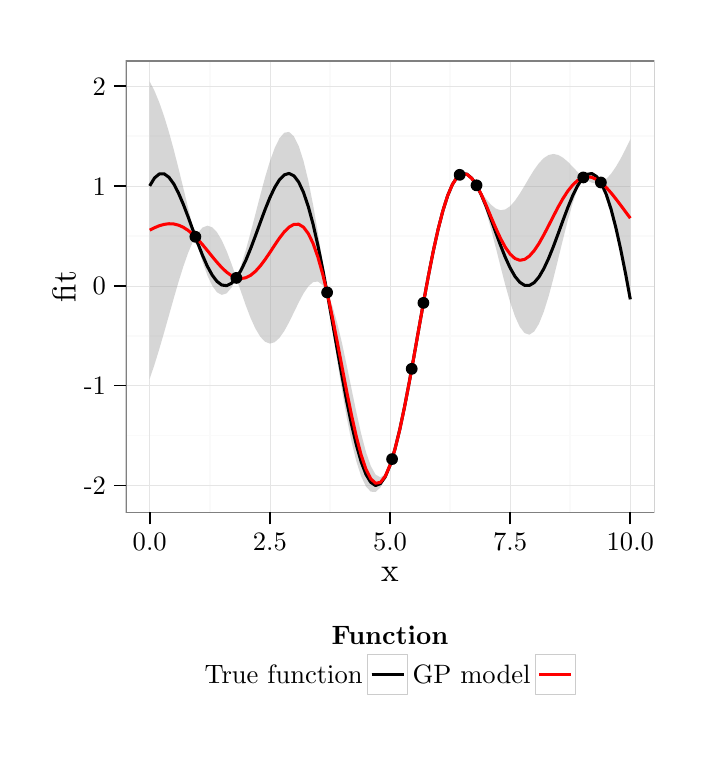
\begin{tikzpicture}[x=1pt,y=1pt]
\definecolor[named]{fillColor}{rgb}{1.00,1.00,1.00}
\path[use as bounding box,fill=fillColor,fill opacity=0.00] (0,0) rectangle (238.49,260.17);
\begin{scope}
\path[clip] (  0.00,  0.00) rectangle (238.49,260.17);
\definecolor[named]{drawColor}{rgb}{1.00,1.00,1.00}
\definecolor[named]{fillColor}{rgb}{1.00,1.00,1.00}

\path[draw=drawColor,line width= 0.6pt,line join=round,line cap=round,fill=fillColor] (  0.00,  0.00) rectangle (238.49,260.17);
\end{scope}
\begin{scope}
\path[clip] ( 35.42, 85.00) rectangle (226.45,248.13);
\definecolor[named]{fillColor}{rgb}{1.00,1.00,1.00}

\path[fill=fillColor] ( 35.42, 85.00) rectangle (226.45,248.13);
\definecolor[named]{drawColor}{rgb}{0.98,0.98,0.98}

\path[draw=drawColor,line width= 0.6pt,line join=round] ( 35.42,112.77) --
	(226.45,112.77);

\path[draw=drawColor,line width= 0.6pt,line join=round] ( 35.42,148.86) --
	(226.45,148.86);

\path[draw=drawColor,line width= 0.6pt,line join=round] ( 35.42,184.95) --
	(226.45,184.95);

\path[draw=drawColor,line width= 0.6pt,line join=round] ( 35.42,221.04) --
	(226.45,221.04);

\path[draw=drawColor,line width= 0.6pt,line join=round] ( 65.81, 85.00) --
	( 65.81,248.13);

\path[draw=drawColor,line width= 0.6pt,line join=round] (109.23, 85.00) --
	(109.23,248.13);

\path[draw=drawColor,line width= 0.6pt,line join=round] (152.64, 85.00) --
	(152.64,248.13);

\path[draw=drawColor,line width= 0.6pt,line join=round] (196.06, 85.00) --
	(196.06,248.13);
\definecolor[named]{drawColor}{rgb}{0.90,0.90,0.90}

\path[draw=drawColor,line width= 0.2pt,line join=round] ( 35.42, 94.72) --
	(226.45, 94.72);

\path[draw=drawColor,line width= 0.2pt,line join=round] ( 35.42,130.81) --
	(226.45,130.81);

\path[draw=drawColor,line width= 0.2pt,line join=round] ( 35.42,166.90) --
	(226.45,166.90);

\path[draw=drawColor,line width= 0.2pt,line join=round] ( 35.42,202.99) --
	(226.45,202.99);

\path[draw=drawColor,line width= 0.2pt,line join=round] ( 35.42,239.08) --
	(226.45,239.08);

\path[draw=drawColor,line width= 0.2pt,line join=round] ( 44.10, 85.00) --
	( 44.10,248.13);

\path[draw=drawColor,line width= 0.2pt,line join=round] ( 87.52, 85.00) --
	( 87.52,248.13);

\path[draw=drawColor,line width= 0.2pt,line join=round] (130.93, 85.00) --
	(130.93,248.13);

\path[draw=drawColor,line width= 0.2pt,line join=round] (174.35, 85.00) --
	(174.35,248.13);

\path[draw=drawColor,line width= 0.2pt,line join=round] (217.76, 85.00) --
	(217.76,248.13);
\definecolor[named]{fillColor}{rgb}{0.60,0.60,0.60}

\path[fill=fillColor,fill opacity=0.40] ( 44.10,240.71) --
	( 45.84,237.29) --
	( 47.58,233.08) --
	( 49.31,228.11) --
	( 51.05,222.40) --
	( 52.79,216.07) --
	( 54.52,209.25) --
	( 56.26,202.14) --
	( 58.00,194.95) --
	( 59.73,187.94) --
	( 61.47,186.02) --
	( 63.21,187.94) --
	( 64.94,188.62) --
	( 66.68,188.04) --
	( 68.42,186.23) --
	( 70.15,183.31) --
	( 71.89,179.45) --
	( 73.63,174.89) --
	( 75.36,169.89) --
	( 77.10,174.26) --
	( 78.84,179.86) --
	( 80.57,186.17) --
	( 82.31,192.87) --
	( 84.05,199.61) --
	( 85.78,206.06) --
	( 87.52,211.85) --
	( 89.26,216.67) --
	( 90.99,220.21) --
	( 92.73,222.21) --
	( 94.47,222.49) --
	( 96.20,220.90) --
	( 97.94,217.40) --
	( 99.67,212.00) --
	(101.41,204.84) --
	(103.15,196.09) --
	(104.88,186.04) --
	(106.62,175.01) --
	(108.36,164.15) --
	(110.09,159.57) --
	(111.83,153.51) --
	(113.57,146.23) --
	(115.30,138.09) --
	(117.04,129.57) --
	(118.78,121.16) --
	(120.51,113.41) --
	(122.25,106.80) --
	(123.99,101.77) --
	(125.72, 98.66) --
	(127.46, 97.67) --
	(129.20, 98.88) --
	(130.93,102.23) --
	(132.67,107.84) --
	(134.41,114.98) --
	(136.14,123.12) --
	(137.88,132.05) --
	(139.62,141.65) --
	(141.35,151.52) --
	(143.09,161.24) --
	(144.83,170.80) --
	(146.56,179.76) --
	(148.30,187.81) --
	(150.04,194.66) --
	(151.77,200.11) --
	(153.51,204.03) --
	(155.25,206.38) --
	(156.98,207.56) --
	(158.72,207.56) --
	(160.46,206.10) --
	(162.19,203.20) --
	(163.93,200.72) --
	(165.67,198.28) --
	(167.40,196.22) --
	(169.14,194.80) --
	(170.88,194.20) --
	(172.61,194.50) --
	(174.35,195.68) --
	(176.08,197.64) --
	(177.82,200.18) --
	(179.56,203.06) --
	(181.29,206.04) --
	(183.03,208.84) --
	(184.77,211.24) --
	(186.50,213.05) --
	(188.24,214.16) --
	(189.98,214.53) --
	(191.71,214.17) --
	(193.45,213.17) --
	(195.19,211.70) --
	(196.92,209.93) --
	(198.66,208.09) --
	(200.40,206.37) --
	(202.13,207.58) --
	(203.87,208.02) --
	(205.61,206.73) --
	(207.34,204.33) --
	(209.08,205.51) --
	(210.82,207.39) --
	(212.55,209.89) --
	(214.29,212.88) --
	(216.03,216.25) --
	(217.76,219.82) --
	(217.76,162.86) --
	(216.03,171.05) --
	(214.29,179.10) --
	(212.55,186.69) --
	(210.82,193.53) --
	(209.08,199.31) --
	(207.34,203.78) --
	(205.61,203.87) --
	(203.87,204.12) --
	(202.13,204.99) --
	(200.40,205.44) --
	(198.66,201.75) --
	(196.92,196.69) --
	(195.19,190.58) --
	(193.45,183.76) --
	(191.71,176.63) --
	(189.98,169.61) --
	(188.24,163.11) --
	(186.50,157.54) --
	(184.77,153.21) --
	(183.03,150.38) --
	(181.29,149.22) --
	(179.56,149.80) --
	(177.82,152.07) --
	(176.08,155.88) --
	(174.35,160.99) --
	(172.61,167.09) --
	(170.88,173.80) --
	(169.14,180.73) --
	(167.40,187.47) --
	(165.67,193.67) --
	(163.93,199.00) --
	(162.19,203.20) --
	(160.46,205.36) --
	(158.72,206.82) --
	(156.98,207.25) --
	(155.25,206.08) --
	(153.51,203.17) --
	(151.77,198.92) --
	(150.04,193.40) --
	(148.30,186.73) --
	(146.56,179.04) --
	(144.83,170.47) --
	(143.09,161.22) --
	(141.35,151.38) --
	(139.62,141.56) --
	(137.88,131.93) --
	(136.14,122.74) --
	(134.41,114.48) --
	(132.67,107.52) --
	(130.93,101.87) --
	(129.20, 97.21) --
	(127.46, 94.02) --
	(125.72, 92.41) --
	(123.99, 92.50) --
	(122.25, 94.35) --
	(120.51, 98.01) --
	(118.78,103.43) --
	(117.04,110.55) --
	(115.30,119.19) --
	(113.57,129.12) --
	(111.83,140.05) --
	(110.09,151.61) --
	(108.36,163.40) --
	(106.62,167.11) --
	(104.88,168.43) --
	(103.15,168.23) --
	(101.41,166.70) --
	( 99.67,164.14) --
	( 97.94,160.88) --
	( 96.20,157.29) --
	( 94.47,153.74) --
	( 92.73,150.57) --
	( 90.99,148.09) --
	( 89.26,146.51) --
	( 87.52,146.02) --
	( 85.78,146.68) --
	( 84.05,148.50) --
	( 82.31,151.40) --
	( 80.57,155.22) --
	( 78.84,159.75) --
	( 77.10,164.74) --
	( 75.36,169.64) --
	( 73.63,166.23) --
	( 71.89,164.18) --
	( 70.15,163.61) --
	( 68.42,164.53) --
	( 66.68,166.91) --
	( 64.94,170.63) --
	( 63.21,175.52) --
	( 61.47,181.38) --
	( 59.73,182.94) --
	( 58.00,178.85) --
	( 56.26,173.92) --
	( 54.52,168.36) --
	( 52.79,162.39) --
	( 51.05,156.23) --
	( 49.31,150.07) --
	( 47.58,144.11) --
	( 45.84,138.48) --
	( 44.10,133.29) --
	cycle;

\path[] ( 44.10,187.00) --
	( 45.84,187.88) --
	( 47.58,188.60) --
	( 49.31,189.09) --
	( 51.05,189.32) --
	( 52.79,189.23) --
	( 54.52,188.81) --
	( 56.26,188.03) --
	( 58.00,186.90) --
	( 59.73,185.44) --
	( 61.47,183.70) --
	( 63.21,181.73) --
	( 64.94,179.63) --
	( 66.68,177.47) --
	( 68.42,175.38) --
	( 70.15,173.46) --
	( 71.89,171.82) --
	( 73.63,170.56) --
	( 75.36,169.76) --
	( 77.10,169.50) --
	( 78.84,169.81) --
	( 80.57,170.69) --
	( 82.31,172.13) --
	( 84.05,174.06) --
	( 85.78,176.37) --
	( 87.52,178.93) --
	( 89.26,181.59) --
	( 90.99,184.15) --
	( 92.73,186.39) --
	( 94.47,188.11) --
	( 96.20,189.09) --
	( 97.94,189.14) --
	( 99.67,188.07) --
	(101.41,185.77) --
	(103.15,182.16) --
	(104.88,177.24) --
	(106.62,171.06) --
	(108.36,163.78) --
	(110.09,155.59) --
	(111.83,146.78) --
	(113.57,137.68) --
	(115.30,128.64) --
	(117.04,120.06) --
	(118.78,112.30) --
	(120.51,105.71) --
	(122.25,100.58) --
	(123.99, 97.14) --
	(125.72, 95.54) --
	(127.46, 95.85) --
	(129.20, 98.05) --
	(130.93,102.05) --
	(132.67,107.68) --
	(134.41,114.73) --
	(136.14,122.93) --
	(137.88,131.99) --
	(139.62,141.60) --
	(141.35,151.45) --
	(143.09,161.23) --
	(144.83,170.64) --
	(146.56,179.40) --
	(148.30,187.27) --
	(150.04,194.03) --
	(151.77,199.51) --
	(153.51,203.60) --
	(155.25,206.23) --
	(156.98,207.40) --
	(158.72,207.19) --
	(160.46,205.73) --
	(162.19,203.20) --
	(163.93,199.86) --
	(165.67,195.98) --
	(167.40,191.85) --
	(169.14,187.76) --
	(170.88,184.00) --
	(172.61,180.79) --
	(174.35,178.34) --
	(176.08,176.76) --
	(177.82,176.12) --
	(179.56,176.43) --
	(181.29,177.63) --
	(183.03,179.61) --
	(184.77,182.22) --
	(186.50,185.29) --
	(188.24,188.64) --
	(189.98,192.07) --
	(191.71,195.40) --
	(193.45,198.47) --
	(195.19,201.14) --
	(196.92,203.31) --
	(198.66,204.92) --
	(200.40,205.91) --
	(202.13,206.28) --
	(203.87,206.07) --
	(205.61,205.30) --
	(207.34,204.06) --
	(209.08,202.41) --
	(210.82,200.46) --
	(212.55,198.29) --
	(214.29,195.99) --
	(216.03,193.65) --
	(217.76,191.34);
\definecolor[named]{drawColor}{rgb}{0.00,0.00,0.00}

\path[draw=drawColor,line width= 1.1pt,line join=round] ( 44.10,202.99) --
	( 45.84,205.88) --
	( 47.58,207.32) --
	( 49.31,207.36) --
	( 51.05,206.10) --
	( 52.79,203.71) --
	( 54.52,200.36) --
	( 56.26,196.29) --
	( 58.00,191.74) --
	( 59.73,186.97) --
	( 61.47,182.25) --
	( 63.21,177.83) --
	( 64.94,173.93) --
	( 66.68,170.75) --
	( 68.42,168.46) --
	( 70.15,167.17) --
	( 71.89,166.95) --
	( 73.63,167.80) --
	( 75.36,169.69) --
	( 77.10,172.51) --
	( 78.84,176.13) --
	( 80.57,180.36) --
	( 82.31,184.99) --
	( 84.05,189.77) --
	( 85.78,194.44) --
	( 87.52,198.74) --
	( 89.26,202.42) --
	( 90.99,205.23) --
	( 92.73,206.98) --
	( 94.47,207.50) --
	( 96.20,206.65) --
	( 97.94,204.37) --
	( 99.67,200.64) --
	(101.41,195.50) --
	(103.15,189.06) --
	(104.88,181.45) --
	(106.62,172.89) --
	(108.36,163.61) --
	(110.09,153.89) --
	(111.83,144.03) --
	(113.57,134.34) --
	(115.30,125.13) --
	(117.04,116.71) --
	(118.78,109.34) --
	(120.51,103.29) --
	(122.25, 98.74) --
	(123.99, 95.86) --
	(125.72, 94.73) --
	(127.46, 95.41) --
	(129.20, 97.87) --
	(130.93,102.01) --
	(132.67,107.71) --
	(134.41,114.77) --
	(136.14,122.96) --
	(137.88,132.00) --
	(139.62,141.60) --
	(141.35,151.45) --
	(143.09,161.23) --
	(144.83,170.65) --
	(146.56,179.41) --
	(148.30,187.27) --
	(150.04,194.02) --
	(151.77,199.50) --
	(153.51,203.58) --
	(155.25,206.22) --
	(156.98,207.42) --
	(158.72,207.23) --
	(160.46,205.77) --
	(162.19,203.20) --
	(163.93,199.72) --
	(165.67,195.55) --
	(167.40,190.95) --
	(169.14,186.17) --
	(170.88,181.48) --
	(172.61,177.13) --
	(174.35,173.34) --
	(176.08,170.30) --
	(177.82,168.17) --
	(179.56,167.06) --
	(181.29,167.02) --
	(183.03,168.05) --
	(184.77,170.10) --
	(186.50,173.07) --
	(188.24,176.80) --
	(189.98,181.12) --
	(191.71,185.79) --
	(193.45,190.57) --
	(195.19,195.20) --
	(196.92,199.41) --
	(198.66,202.96) --
	(200.40,205.61) --
	(202.13,207.16) --
	(203.87,207.45) --
	(205.61,206.37) --
	(207.34,203.84) --
	(209.08,199.87) --
	(210.82,194.51) --
	(212.55,187.85) --
	(214.29,180.07) --
	(216.03,171.37) --
	(217.76,162.00);
\definecolor[named]{drawColor}{rgb}{1.00,0.00,0.00}

\path[draw=drawColor,line width= 1.1pt,line join=round] ( 44.10,187.00) --
	( 45.84,187.88) --
	( 47.58,188.60) --
	( 49.31,189.09) --
	( 51.05,189.32) --
	( 52.79,189.23) --
	( 54.52,188.81) --
	( 56.26,188.03) --
	( 58.00,186.90) --
	( 59.73,185.44) --
	( 61.47,183.70) --
	( 63.21,181.73) --
	( 64.94,179.63) --
	( 66.68,177.47) --
	( 68.42,175.38) --
	( 70.15,173.46) --
	( 71.89,171.82) --
	( 73.63,170.56) --
	( 75.36,169.76) --
	( 77.10,169.50) --
	( 78.84,169.81) --
	( 80.57,170.69) --
	( 82.31,172.13) --
	( 84.05,174.06) --
	( 85.78,176.37) --
	( 87.52,178.93) --
	( 89.26,181.59) --
	( 90.99,184.15) --
	( 92.73,186.39) --
	( 94.47,188.11) --
	( 96.20,189.09) --
	( 97.94,189.14) --
	( 99.67,188.07) --
	(101.41,185.77) --
	(103.15,182.16) --
	(104.88,177.24) --
	(106.62,171.06) --
	(108.36,163.78) --
	(110.09,155.59) --
	(111.83,146.78) --
	(113.57,137.68) --
	(115.30,128.64) --
	(117.04,120.06) --
	(118.78,112.30) --
	(120.51,105.71) --
	(122.25,100.58) --
	(123.99, 97.14) --
	(125.72, 95.54) --
	(127.46, 95.85) --
	(129.20, 98.05) --
	(130.93,102.05) --
	(132.67,107.68) --
	(134.41,114.73) --
	(136.14,122.93) --
	(137.88,131.99) --
	(139.62,141.60) --
	(141.35,151.45) --
	(143.09,161.23) --
	(144.83,170.64) --
	(146.56,179.40) --
	(148.30,187.27) --
	(150.04,194.03) --
	(151.77,199.51) --
	(153.51,203.60) --
	(155.25,206.23) --
	(156.98,207.40) --
	(158.72,207.19) --
	(160.46,205.73) --
	(162.19,203.20) --
	(163.93,199.86) --
	(165.67,195.98) --
	(167.40,191.85) --
	(169.14,187.76) --
	(170.88,184.00) --
	(172.61,180.79) --
	(174.35,178.34) --
	(176.08,176.76) --
	(177.82,176.12) --
	(179.56,176.43) --
	(181.29,177.63) --
	(183.03,179.61) --
	(184.77,182.22) --
	(186.50,185.29) --
	(188.24,188.64) --
	(189.98,192.07) --
	(191.71,195.40) --
	(193.45,198.47) --
	(195.19,201.14) --
	(196.92,203.31) --
	(198.66,204.92) --
	(200.40,205.91) --
	(202.13,206.28) --
	(203.87,206.07) --
	(205.61,205.30) --
	(207.34,204.06) --
	(209.08,202.41) --
	(210.82,200.46) --
	(212.55,198.29) --
	(214.29,195.99) --
	(216.03,193.65) --
	(217.76,191.34);
\definecolor[named]{fillColor}{rgb}{0.00,0.00,0.00}

\path[fill=fillColor] (207.13,204.23) circle (  2.13);

\path[fill=fillColor] (138.77,136.89) circle (  2.13);

\path[fill=fillColor] (162.19,203.20) circle (  2.13);

\path[fill=fillColor] (200.77,206.04) circle (  2.13);

\path[fill=fillColor] (143.00,160.72) circle (  2.13);

\path[fill=fillColor] (156.10,206.99) circle (  2.13);

\path[fill=fillColor] (131.68,104.28) circle (  2.13);

\path[fill=fillColor] ( 75.41,169.75) circle (  2.13);

\path[fill=fillColor] ( 60.60,184.61) circle (  2.13);

\path[fill=fillColor] (108.20,164.50) circle (  2.13);
\definecolor[named]{drawColor}{rgb}{0.50,0.50,0.50}

\path[draw=drawColor,line width= 0.6pt,line join=round,line cap=round] ( 35.42, 85.00) rectangle (226.45,248.13);
\end{scope}
\begin{scope}
\path[clip] (  0.00,  0.00) rectangle (238.49,260.17);
\definecolor[named]{drawColor}{rgb}{0.00,0.00,0.00}

\node[text=drawColor,anchor=base east,inner sep=0pt, outer sep=0pt, scale=  0.96] at ( 28.31, 91.42) {-2};

\node[text=drawColor,anchor=base east,inner sep=0pt, outer sep=0pt, scale=  0.96] at ( 28.31,127.51) {-1};

\node[text=drawColor,anchor=base east,inner sep=0pt, outer sep=0pt, scale=  0.96] at ( 28.31,163.60) {0};

\node[text=drawColor,anchor=base east,inner sep=0pt, outer sep=0pt, scale=  0.96] at ( 28.31,199.69) {1};

\node[text=drawColor,anchor=base east,inner sep=0pt, outer sep=0pt, scale=  0.96] at ( 28.31,235.78) {2};
\end{scope}
\begin{scope}
\path[clip] (  0.00,  0.00) rectangle (238.49,260.17);
\definecolor[named]{drawColor}{rgb}{0.00,0.00,0.00}

\path[draw=drawColor,line width= 0.6pt,line join=round] ( 31.15, 94.72) --
	( 35.42, 94.72);

\path[draw=drawColor,line width= 0.6pt,line join=round] ( 31.15,130.81) --
	( 35.42,130.81);

\path[draw=drawColor,line width= 0.6pt,line join=round] ( 31.15,166.90) --
	( 35.42,166.90);

\path[draw=drawColor,line width= 0.6pt,line join=round] ( 31.15,202.99) --
	( 35.42,202.99);

\path[draw=drawColor,line width= 0.6pt,line join=round] ( 31.15,239.08) --
	( 35.42,239.08);
\end{scope}
\begin{scope}
\path[clip] (  0.00,  0.00) rectangle (238.49,260.17);
\definecolor[named]{drawColor}{rgb}{0.00,0.00,0.00}

\path[draw=drawColor,line width= 0.6pt,line join=round] ( 44.10, 80.73) --
	( 44.10, 85.00);

\path[draw=drawColor,line width= 0.6pt,line join=round] ( 87.52, 80.73) --
	( 87.52, 85.00);

\path[draw=drawColor,line width= 0.6pt,line join=round] (130.93, 80.73) --
	(130.93, 85.00);

\path[draw=drawColor,line width= 0.6pt,line join=round] (174.35, 80.73) --
	(174.35, 85.00);

\path[draw=drawColor,line width= 0.6pt,line join=round] (217.76, 80.73) --
	(217.76, 85.00);
\end{scope}
\begin{scope}
\path[clip] (  0.00,  0.00) rectangle (238.49,260.17);
\definecolor[named]{drawColor}{rgb}{0.00,0.00,0.00}

\node[text=drawColor,anchor=base,inner sep=0pt, outer sep=0pt, scale=  0.96] at ( 44.10, 71.27) {0.0};

\node[text=drawColor,anchor=base,inner sep=0pt, outer sep=0pt, scale=  0.96] at ( 87.52, 71.27) {2.5};

\node[text=drawColor,anchor=base,inner sep=0pt, outer sep=0pt, scale=  0.96] at (130.93, 71.27) {5.0};

\node[text=drawColor,anchor=base,inner sep=0pt, outer sep=0pt, scale=  0.96] at (174.35, 71.27) {7.5};

\node[text=drawColor,anchor=base,inner sep=0pt, outer sep=0pt, scale=  0.96] at (217.76, 71.27) {10.0};
\end{scope}
\begin{scope}
\path[clip] (  0.00,  0.00) rectangle (238.49,260.17);
\definecolor[named]{drawColor}{rgb}{0.00,0.00,0.00}

\node[text=drawColor,anchor=base,inner sep=0pt, outer sep=0pt, scale=  1.20] at (130.93, 60.00) {x};
\end{scope}
\begin{scope}
\path[clip] (  0.00,  0.00) rectangle (238.49,260.17);
\definecolor[named]{drawColor}{rgb}{0.00,0.00,0.00}

\node[text=drawColor,rotate= 90.00,anchor=base,inner sep=0pt, outer sep=0pt, scale=  1.20] at ( 17.30,166.56) {fit};
\end{scope}
\begin{scope}
\path[clip] (  0.00,  0.00) rectangle (238.49,260.17);
\definecolor[named]{fillColor}{rgb}{1.00,1.00,1.00}

\path[fill=fillColor] ( 59.67, 14.89) rectangle (202.20, 48.12);
\end{scope}
\begin{scope}
\path[clip] (  0.00,  0.00) rectangle (238.49,260.17);
\definecolor[named]{drawColor}{rgb}{0.00,0.00,0.00}

\node[text=drawColor,anchor=base,inner sep=0pt, outer sep=0pt, scale=  0.96] at (130.93, 37.23) {\bfseries Function};
\end{scope}
\begin{scope}
\path[clip] (  0.00,  0.00) rectangle (238.49,260.17);
\definecolor[named]{drawColor}{rgb}{0.80,0.80,0.80}
\definecolor[named]{fillColor}{rgb}{1.00,1.00,1.00}

\path[draw=drawColor,line width= 0.6pt,line join=round,line cap=round,fill=fillColor] (122.82, 19.16) rectangle (137.28, 33.61);
\end{scope}
\begin{scope}
\path[clip] (  0.00,  0.00) rectangle (238.49,260.17);
\definecolor[named]{drawColor}{rgb}{0.00,0.00,0.00}

\path[draw=drawColor,line width= 1.1pt,line join=round] (124.27, 26.39) -- (135.83, 26.39);
\end{scope}
\begin{scope}
\path[clip] (  0.00,  0.00) rectangle (238.49,260.17);
\definecolor[named]{drawColor}{rgb}{0.00,0.00,0.00}

\path[draw=drawColor,line width= 1.1pt,line join=round] (124.27, 26.39) -- (135.83, 26.39);
\end{scope}
\begin{scope}
\path[clip] (  0.00,  0.00) rectangle (238.49,260.17);
\definecolor[named]{drawColor}{rgb}{0.80,0.80,0.80}
\definecolor[named]{fillColor}{rgb}{1.00,1.00,1.00}

\path[draw=drawColor,line width= 0.6pt,line join=round,line cap=round,fill=fillColor] (183.48, 19.16) rectangle (197.93, 33.61);
\end{scope}
\begin{scope}
\path[clip] (  0.00,  0.00) rectangle (238.49,260.17);
\definecolor[named]{drawColor}{rgb}{1.00,0.00,0.00}

\path[draw=drawColor,line width= 1.1pt,line join=round] (184.92, 26.39) -- (196.49, 26.39);
\end{scope}
\begin{scope}
\path[clip] (  0.00,  0.00) rectangle (238.49,260.17);
\definecolor[named]{drawColor}{rgb}{1.00,0.00,0.00}

\path[draw=drawColor,line width= 1.1pt,line join=round] (184.92, 26.39) -- (196.49, 26.39);
\end{scope}
\begin{scope}
\path[clip] (  0.00,  0.00) rectangle (238.49,260.17);
\definecolor[named]{drawColor}{rgb}{0.00,0.00,0.00}

\node[text=drawColor,anchor=base west,inner sep=0pt, outer sep=0pt, scale=  0.96] at ( 63.93, 23.08) {True function};
\end{scope}
\begin{scope}
\path[clip] (  0.00,  0.00) rectangle (238.49,260.17);
\definecolor[named]{drawColor}{rgb}{0.00,0.00,0.00}

\node[text=drawColor,anchor=base west,inner sep=0pt, outer sep=0pt, scale=  0.96] at (139.08, 23.08) {GP model};
\end{scope}
\end{tikzpicture}

  %\includegraphics[width=8cm]{gp_example}
  \caption{
    The Gaussian process interpolation of the function 
    $f(x) = sin(x) + cos(2x)$ from 10 uniformly distributed samples.  
    The standard error of estimation from the model is shown in gray.
    Note that the standard error increases with the distance from the sample
    points.
  }
  \label{fig:gp_example}
\end{figure}

Parameterizing a Gaussian process model means correctly parameterizing the 
correlation functions to the data samples.  If the function varies a lot 
between the sample points then we would expect low correlation between the
sample points, while if the function is relatively stable between the sample
points then we would expect high correlation between the points.  
In the spatial sense, this high and low correlation can be seen as the 
amount of influence the value of a particular sample point has on the value
at another location a particular distance away.

\subsection{Applications in multi-D}
\label{sec:gp_applications}

Gaussian process regression is very common in the statistics community
to analyze simulations among other types of data.
There exist a number of examples where Gaussian process regression along
with a uniformly distributed experimental design is used in order to 
run an analysis.
%By looking at commonalities in terms of dimensions and numbers of points
%for examining these simulations we can determine the order of dimensions
%and number of sample points we need to build our predictive function on.
Using uniform sampling with a Gaussian process model 
has been applied in 
an optimization scenario, as with
Couckuyt et al.~\cite{Couckuyt:2010}.  They used a sparse initial sampling
and then built a GP model to emulate microwave filter and textile antenna
simulations.  They then incrementally ran additional samples of the simulation
in order to find optimal parameter settings.  This process of finding 
additional sample locations can be quite expensive computationally.
Hutter et al.~\cite{Hutter:2010}
develop a method to find new sample locations when under a time budget.
They then applied this method to find optimal parameters for a search
algorithm for a propositional satisfyability solver.
This method was also used to perform
a sensitivity analysis of an arctic sea ice
prediction model~\cite{Chapman:1994}.  They decomposed the Gaussian process
model to find ``average'' behavior due to each model parameter.
Linkletter et al.~\cite{Linkletter:2006} 
used Gaussian process models to measure the sensitivity of parameters to
a cylinder deformation simulation to reduce the parameter space from 14 input 
factors to seven.
Kaufman et al.~\cite{Kaufman:2011} use compactly supported correlation 
functions to build Gaussian process models efficiently on
very large data sets.  This was applied to cosmological data.
Hensman et al.~\cite{Hensman:2013} used an approach to train 
a Gaussian process model on $700,000$ data points in an $8$-dimensional space
to build a model to predict flight delays using a lower rank covariance
matrix.
Shepherd and Owenius~\cite{Shepherd:2012} used Gaussian process models 
as a classification tool in order to classify voxels in dPET images in order
to find tumor sites.

\begin{table*}[htb]
\centering
\caption{
  A summary of the literature described in \autoref{sec:gp_applications}.  We
  show the domain of application of each paper, their analysis goal, as
  well as the number of samples and number of input parameters (dimensions)
  of the simulation used to train the GP model. 
}
\begin{tabular}{|r|lrrl|}
  \hline
  Reference & Application & Dimensions & Samples & Goal \\
  \hline
  Couckuyt et al.~\cite{Couckuyt:2010} & Microwave filter & 5 & 51 & Optimization \\
  Couckuyt et al.~\cite{Couckuyt:2010} & Textile antenna & 2 & 14 & Optimization \\
  Hutter et al.~\cite{Hutter:2010} & Propositional logic satisfyability & 4 & 25 & Optimization \\
  Chapman et al.~\cite{Chapman:1994} & Sea ice prediction & 13 & 157 & Sensitivity analysis \\
  Linkletter et al.~\cite{Linkletter:2006} & Cylinder deformation model & 14 & 118 & Sensitivity analysis \\
  Kaufman et al.~\cite{Kaufman:2011} & Cosmological data  & 4 & 20,000 & Prediction \\
  Hensman et al.~\cite{Hensman:2013} & Flight delays & 8 & 700,000 & Prediction \\
  Shepherd and Owenius~\cite{Shepherd:2012} & dPET data in radiation oncology & 4 & 6 patient images & Classification \\
  \hline
\end{tabular}
\label{tb:literature}
\end{table*}

As one can see, there are a wide variety of application domains.  However, 
all these analyses share commonalities.
We show the summary information of these studies in \autoref{tb:literature}.
The number of inputs is typically on
the order of 5--15 inputs. Each of these may correspond to a known factor that
can vary in the real world like wind speed or the velocity of a particle, or
an unknown fixed-quantity in the real world like Planck's constant or the
gravitational constant.  The simulation code typically creates a complex
object like a 3D+time model of the world or a segmented image. On these
outputs scientists define a number of feature extractors or objective
functions which reduce the complex output to a set of numerical 
attributes~\cite{Sedlmair:2014}.
Therefore, for each simulation run we get a vector of scalar input factors and
the corresponding vector of scalar outputs.  Each scalar output can be
considered in a separate analysis so in this paper we assume that there is
only one scalar output for each input configuration.

The practical number of simulation samples range from a few hundred to hundreds
of thousands.  This is due to either time or monetary constraints.  Running more
simulations than this simply takes too long or costs too much.  
Based on these
data we test our timing function on dimensions $3$--$8$ and run up to 
$1,000,000$ sample points.


\subsection{Pipeline description}

Despite the wide variety of application areas, all the simulation studies 
mentioned follow a standard procedure for
analysis.
They start with a uniform sampling of the parameter space. This is
usually done with a space-filling
design like a Latin 
hypercube~\cite{Mckay:1979}, Halton
sequence~\cite{Halton:1964}, or Centroidal Voronoi tesselation~\cite{Du:1999}. 
Without any knowledge of the relative
importance of the dimensions they are sampled equally.

The
simulation is run using each sample and the outputs are recorded. If the
output is a complex object then feature
extractors are run on the outputs to generate scalar results.
We then build an emulator of this
process. Prediction using this emulator must be fast as we will want to
evaluate it at many points. Often, a Gaussian process
model~\cite{Rasmussen:2006} is selected for the emulator. 

\begin{figure}[htb]
  \centering
  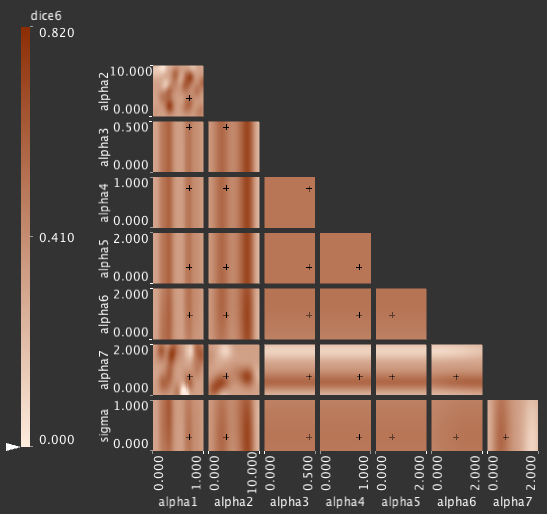
\includegraphics[width=7cm]{tuner}
  \caption[Tuner's HyperSlice view]{\
    Screenshot of Tuner~\cite{Torsney-Weir:2011} demonstrating the
    HyperSlice~\cite{Wijk:1993} method for rendering an
    $8$-dimensional parameter space using squared exponential kernel 
    reconstruction on an image segmentation dataset.
    Here we show the view using the conditional mean of the Gaussian 
    process model.
  } 
  \label{fig:tuner}
\end{figure}

With this emulator the user can now analyze the input\slash output
relationship of the simulation. This can be done in a variety of ways, either by
looking at static plots~\cite{Chapman:1994} or by interactively exploring the
response surface~\cite{Torsney-Weir:2011}. We show an example of the
HyperSlice technique for interactively exploring the response surface
as implemented in Tuner~\cite{Torsney-Weir:2011} in \autoref{fig:tuner}.  
In this case we show the conditional mean of the Gaussian process model.
Tuner can also show the estimation variability if desired.

Interactive 
exploration of the Gaussian process model is a 
relatively new technique as it is more complex to implement and the limits
in terms of the number of points and how the size of the kernels affects 
interactivity is not yet understood.  
The rest of this paper will discuss how to address both these questions.
We present a rendering algorithm which is similar to 
splatting~\cite{Mueller:1998}
to render the Gaussian
process prediction function using HyperSlice.
We also develop a method to determine when
the interactivity of the rendering will fail taking into account the geometric 
interpretation of the Gaussian process model as well as the performance
of an individual user's machine.

